\chapter{Movimiento relativo}

\begin{miparrafo}

En mecánica newtoniana, un sistema de referencia inercial es un sistema de referencia en el que las leyes del movimiento cumplen las leyes de Newton y, por tanto, la variación del momento lineal del sistema es igual a las fuerzas reales sobre el sistema, es decir, un sistema en el que:
$\quad \vec F_{real} = \displaystyle \dv{\vec p}{t}$


\vspace{2mm} En cambio, la descripción newtoniana de un sistema no inercial requiere la introducción de fuerzas ficticias o inerciales, de tal manera que:
$\quad \displaystyle \dv{\vec p}{t}=\vec {F} _{real}-\vec {F}_{fict}$

\vspace{2mm} Esto lleva a una definición alternativa, un sistema inercial es aquel en que el movimiento de las partículas puede describirse empleando solo fuerzas reales sin necesidad de considerar fuerzas ficticias.

\vspace{2mm} El concepto de sistema de referencia inercial también es aplicable a teorías más generales que la mecánica newtoniana. Así, en la teoría de la relatividad especial también se pueden introducir los sistemas inerciales. Aunque en relatividad especial la caracterización matemática no coincide con la que se da en mecánica newtoniana, debido a que la segunda ley de Newton, tal como la formuló, no se cumple en la Teoría de la relatividad. El concepto de sistema de referencia no fue establecido hasta dos siglos después de la formulación de las leyes de Newton (1687), cuando Ludwig Lange (1885) introdujo el concepto en un intento de eliminar la necesidad de un espacio y un tiempo absolutos del tipo que Newton conjeturaba. Estas ideas fueron, poco más tarde, consideradas en la formulación de la teoría de la relatividad especial.
	
\end{miparrafo}

%\vspace{35mm} %********************

\section{Sistema de Referencia inercial}

\begin{multicols}{2}
	
$\displaystyle \vec v_A=\dv{\vec r_A}{t}; \qquad \vec v_B=\dv{\vec r_B}{t}$

$\quad$

$\vec r_{AB}=\vec r_B-\vec r_A$

$\quad$

?`Con que \emph{velocidad relativa} se mueve una partícula respecto de la otra?


\begin{figure}[H]
	\centering
	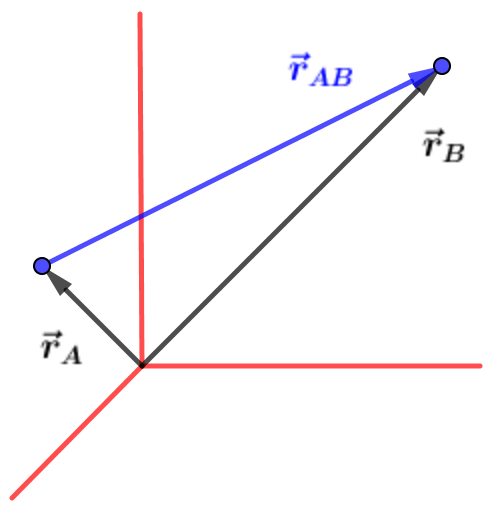
\includegraphics[width=.35\textwidth]{imagenes/imagenes10/T10IM01.png}
\end{figure}	
\end{multicols}

$\vec v_{AB}=\displaystyle \dv{\vec r_{AB}}{t}=\dv{\vec r_B-\vec r_A}{t}=\vec v_B-\vec v_A$

Análogamente: $\vec v_{BA}=\vec v_B-\vec v_A \to\ $ conclusión: 

\begin{equation}
\boldsymbol{ \vec v_{AB}=-\vec v_{BA} }	
\end{equation}

Derivando respecto al tiempo: $\quad \vec a_{AB}=-\vec a_{BA}$

\section[Movimiento de traslación uniforme. Principio de la relatividad de Galileo]{Movimiento de traslación uniforme. Principio de la relatividad de Galileo\sectionmark{Principio de relatividad de Galileo}}
\sectionmark{Principio de relatividad de Galileo}
\begin{multicols}{2}
Supongamos dos observadores $\mathcal O$ y $\mathcal O'$ que se mueven, uno respecto al otro, con velocidad uniforme $\vec V=\overrightarrow{cte}$, velocidad constante en módulo y dirección ( y sentido).

En $t=0$ los origenes coinciden, $\mathcal O \equiv \mathcal O'$.
\begin{figure}[H]
	\centering
	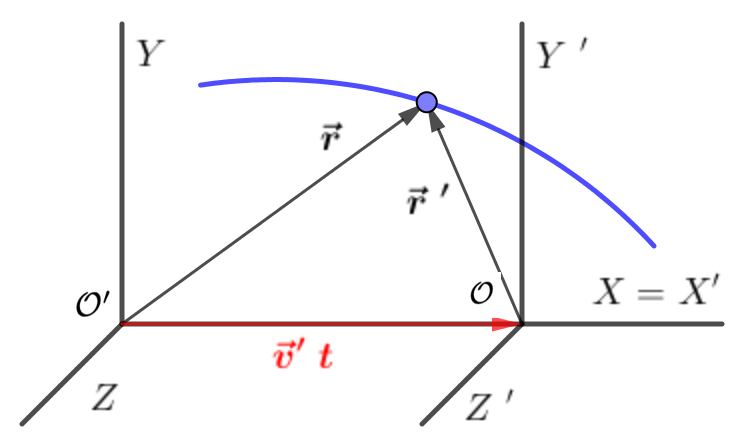
\includegraphics[width=.5\textwidth]{imagenes/imagenes10/T10IM02.png}
\end{figure}
\end{multicols}
$\mathcal O$, observa una partícula en movimiento. ?`Cómo debe pasarle la información a $\mathcal O'$?

\begin{equation}
\subrayado{\vec r=\vec V \ t + \vec r \ '} \quad \text{Transformación de Galileo de posiciones}	
\end{equation}

derivando respecto al tiempo,

\begin{equation}
\subrayado{\vec v=\vec V \ t + \vec v \ '} \quad \text{Transformación de Galileo de velocidades}	
\end{equation}

si volvemos a derivar respecto del tiempo,

\begin{equation}
\subrayado{\vec a= \vec a \ '} \qquad \qquad \textcolor{gris}{\vec V=\overrightarrow{cte}\to \dv{\vec V}{t}=0}	
\end{equation}

Como la masa es invariante (no depende de $t$), \emph{``las leyes de la dinámica son las mismas en ambos sistemas.''}

En tres dimensiones, si es $X$ el eje de movimiento de $\mathcal O$ respecto de $\mathcal O'$:

\begin{equation}
\begin{cases}
\ \subrayado{x=Vt+x'} \\ \  \subrayado{y=y'} \\ \  \subrayado{z=z'}	
\end{cases}
\qquad \qquad 
\begin{cases}
\  \subrayado{v_x=V+v'_x} \\ \ \subrayado{v_y=v'_y} \\ \ \subrayado{v_z=v'_z}	
\end{cases}	
\end{equation}


\textbf{Principio de relatividad de Galileo:} \emph{``Cuando se tienen dos sistemas de referencia que se desplazan uno respecto del otro a velocidad uniforme, \colorbox{LightYellow}{las leyes de la dinámica} son las mismas en ambos sistemas.''}

Newton pone su sistema de referencia en las `estrellas fijas', le llama \emph{``sistema de referencia inercial.''}. En todos los infinitos sistemas de referencia que se muevan con $\vec V=\overrightarrow{cte}$ respecto del `sistema inercial de Newton' son válidas las leyes de Newton (dinámica).

Como la tierra gira, $\vec V \neq \overrightarrow{cte}$ respecto del sistema inercial de Newton, no serán válidas las leyes de Newton, las tendremos que transformar.

\section{Operador derivada respecto a $t$}

\textbf{Operador derivada respecto del tiempo en el cambio de sistemas de referencia en rotación.}

\begin{multicols}{2}
Ambos observadores $\mathcal O \text{ y } \mathcal O'$, sistemas de referencia, giran uno respecto al otro con velocidad angular $\vec \omega$, sin desplazarse.

Sea $\vec A$ un vector cualquiera:

Medido por $\mathcal O$:

$\vec A=\vec i A_x+\vec j A_y+ \vec k A_z$

Medido por $\mathcal O'$:

$\vec A=\vec i\ ' A'_x+\vec j\ ' A'_y+ \vec k\ ' A'_z$
\begin{figure}[H]
	\centering
	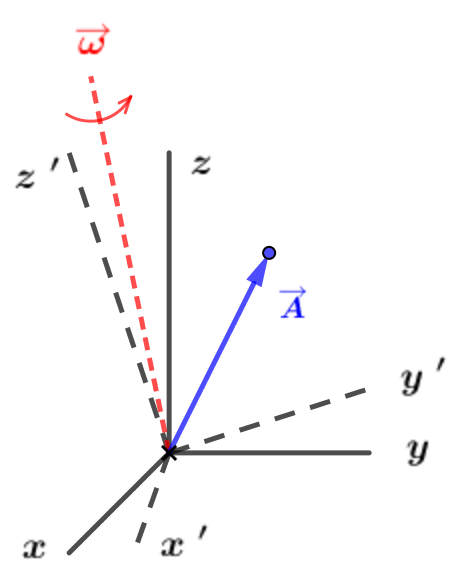
\includegraphics[width=.4\textwidth]{imagenes/imagenes10/T10IM03.png}
\end{figure}
\end{multicols}

El observador $\mathcal O$ mide como varía $\vec A$ respecto del tiempo:

$\displaystyle \left( \dv{\vec A}{t} \right)_{\mathcal O}=
\left[ \dv{t} \left( \vec i\ ' A'_x+\vec j\ ' A'_y+ \vec kº ' A'_z \right) \right]_{\mathcal O} =$

$= \displaystyle \left[ \vec i\ ' \dv{A_x}{t} + \vec j\ ' \dv{A_y}{t} + \vec k\ ' \dv{A_z}{t} \right] \ + \ 
\left[ A'_x \dv{\vec i\ '}{t} + A'_y \dv{\vec j\ '}{t} + A'_z \dv{\vec k\ '}{t} \right] =$

$= \displaystyle  \left( \dv{\vec A}{t} \right)_{\mathcal O'} \ + \ 
\left[ A'_x \dv{\vec i\ '}{t} + A'_y \dv{\vec j\ '}{t} + A'_z \dv{\vec k\ '}{t} \right] $

Como $\displaystyle A'_x \dv{\vec i\ '}{t} + A'_y \dv{\vec j\ '}{t} + A'_z \dv{\vec k\ '}{t}= A'_x\ \vec \omega \times \vec i + A'_y\ \vec \omega \times \vec j + A'_z\ \vec \omega \times \vec k$,

\begin{equation}
	\boldsymbol{ \left( \dv{\vec A}{t} \right)_{\mathcal O}=\left( \dv{\vec A}{t} \right)_{\mathcal O'}+\vec \omega \times \vec A }
\end{equation}

Escrito en forma de \emph{operador matemático:}

$$\boldsymbol{ \left( \dv{t}\right)_{\mathcal O} =  \left( \dv{t}\right)_{\mathcal O'} + \vec \omega \times \underline{\ \ }  }$$

\section{Movimiento relativo rotacional}

Ambos observadores $\mathcal O \text{ y } \mathcal O'$, sistemas de referencia, giran uno respecto al otro con velocidad angular $\vec \omega$, sin desplazarse. 

Ambos miden el mismo vector de posición da una partícula en movimiento en un tiempo $t$: $ \ \  \vec r = \vec r'$. Veamos que ocurre con las velocidades.

$$\displaystyle \vec v = \left( \dv{\vec r}{t} \right)_{\mathcal O}=
\left( \dv{\vec r}{t} \right)_{\mathcal O'} + \vec \omega \times \vec r$$

$$ \boldsymbol{ \vec v = \vec v \ ' + \vec \omega \times \vec r } $$

Relación entre las velocidades $\vec v$ y $\vec v'$ de un mismo punto material que miden dos observadores que están girando uno respecto del otro con velocidad angular $\vec \omega$ pero sin separarse.
  
Derivando respecto del tiempo:

$\vec a = \displaystyle \left( \dv{\vec v}{t} \right)_{\mathcal O} =  \left( \dv{\vec v}{t} \right)_{\mathcal O'}+ \vec \omega \times \vec v \ $ \textcolor{gris}{ Aplicando el operador derivada respecto del tiempo para sistemas de referencia en rotación.}

Por otra parte, \textcolor{gris}{teniendo en cuenta la expresión anterior $\vec v = \vec v \ ' + \vec \omega \times \vec r$}:

$\displaystyle \vec a = \left[ \dv{t} (\  \vec v \ ' + \vec \omega \times \vec r \ ) \right]_{\mathcal O'} + \vec \omega \times (\  \vec v \ ' + \vec \omega \times \vec r \ ) = $

$\displaystyle = \left( \dv{\vec v\ '}{t} \right)_{\mathcal O'}+ \left(  \dv{\vec \omega}{t}\right)_{\mathcal O'} + \left( \dv{\vec r}{t} \right)_{\mathcal O'} \times \vec r +
\vec w \times \vec v\ ' + \vec \omega \times ( \ \vec \omega  \times  \vec r \ )$

Como $\ \vec r=\vec r\ ' \ \to \ \displaystyle \left( \dv{\vec r}{t} \right)_{\mathcal O'} =\left( \dv{\vec r \ '}{t} \right)_{\mathcal O'} = \vec v\ '$


$$\boldsymbol{ \displaystyle \vec a = \vec a\ ' + \dot{\vec \omega} \times \vec r + 2 \vec \omega \times \vec v\ '+ \vec \omega \times ( \ \vec \omega  \times  \vec r) }$$

Siendo $ \ \dot{\vec \omega}=\displaystyle \dv{\vec \omega}{t}$

--- El término $\dot{\vec \omega} \times \vec r$ no figura cuando $\vec \omega=\overrightarrow{cte}$.

--- El término $2\vec \omega \times \vec v\ '$ recibe el nombre de \textbf{\emph{aceleración de coriolis.}}

--- El último término, $\vec \omega (\ \vec \omega \times \vec r \ )$, es la \textbf{\emph{aceleración centrípeta}}, apunta hacia el eje de movimiento ($\vec \omega$).

Nota: El paréntesis en $\vec \omega \times ( \ \vec \omega  \times  \vec r \ )$ es muy importante pues \textbf{el producto vectorial no es}, \emph{afortunadamente}, \textbf{asociativo}. $\quad$ ;-)

\begin{figure}[H]
	\centering
	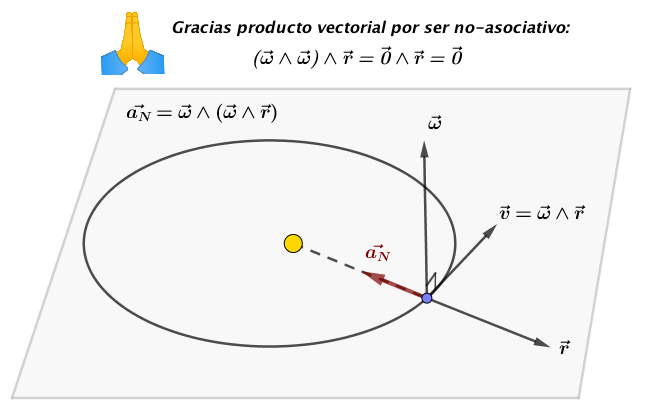
\includegraphics[width=.9\textwidth]{imagenes/imagenes02/T02IM33.png}
\end{figure}


Si $\mathcal O$ es un observador inercial $\to \mathcal O'$ no será un observador inercial, para él no serán válidas las leyes de Newton, despejando $\vec a \ '  $:

$ \displaystyle m \cdot \vec a\ ' =  m \cdot \vec a -  m \cdot \dot{\vec \omega} \times \vec r - 2  m \cdot \vec \omega \times \vec v\ '-  m \cdot \vec \omega \times ( \ \vec \omega  \times  \vec r) $


Si consideramos $\ \vec \omega=\overrightarrow{cte}$ queda

$ \displaystyle m \cdot \vec a\ ' =  m \cdot \vec a -  \cancelto{0}{m \cdot \dot{\vec \omega} \times \vec r} - 2  m \cdot \vec \omega \times \vec v\ '-  m \cdot \vec \omega \times ( \ \vec \omega  \times  \vec r) $,

$\vec F \ '= \vec F + \vec F_{\text{coriolis}}+ \vec F_{\text{centrípeta}}$

\begin{miparrafodestacado}
	 Ambas nuevas fuerzas que ahora aparecen, la \emph{fuerza de coriolis} y la \emph{fuerza centrífuga}, son \emph{fuerzas de inercia} que no tienen existencia real y solo se manifiestan cuando elegimos un sistema de referencia no inercial.
\end{miparrafodestacado}


\section{Movimiento relativo general}

Los dos observadores que desean intercambiar información, además de girar, se trasladan.

\begin{multicols}{2}
$\vec r=\vec h + \vec r\ '$

$\vec v=\displaystyle \left( \dv{\vec r}{t} \right)_{\mathcal O}=
\left( \dv{\vec h}{t} \right)_{\mathcal O} + \left( \dv{\vec r\ '}{t} \right)_{\mathcal O}$

Utilizado el operador derivada respecto del tiempo visto anteriormente,

$\vec v=\displaystyle \left( \dv{\vec h}{t} \right)_{\mathcal O} + \left( \dv{\vec r \ '}{t} \right)_{\mathcal O'}+\vec \omega \times \vec r \ '$

\begin{figure}[H]
	\centering
	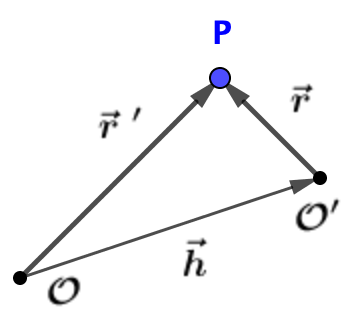
\includegraphics[width=.3\textwidth]{imagenes/imagenes10/T10IM04.png}
\end{figure}
\end{multicols}

$\vec v=\displaystyle \left( \dv{\vec h}{t} \right)_{\mathcal O} + \left( \dv{\vec r \ '}{t} \right)_{\mathcal O'}+\vec \omega \times \vec r \ '$

El primer término del segundo miembro responde a una traslación y los otros dos términos a una rotación.

Cualquier movimiento arbitrario se puede descomponer como un movimiento de  traslación y un movimiento de rotación.

$$\boldsymbol{ \displaystyle \vec v=\vec v\ ' + \vec \omega \times \vec r\ '+  \left( \dv{\vec h}{t} \right)_{\mathcal O} }$$


Derivando respecto al tiempo,

$\vec a= \left( \displaystyle \dv{\vec v}{t} \right)_{\mathcal O}=
\left\{  
\displaystyle \dv{t} \left[
\vec v \ ' + \vec \omega \times \vec r\ ' + \left( \dv{\vec h}{t} \right)_{\mathcal O}
\right]
\right\}_{\mathcal{O}}$

Teniendo en cuenta el operador derivada respecto al tiempo en rotaciones,

$$\boldsymbol{ 
\vec a = \vec a\ ' + 2 \vec \omega \times \vec v\ '+ \dot{\vec \omega}\times \vec r \ ' + \vec \omega \times (\vec \omega \times \vec r \ ')+ \left( \displaystyle \dv[2]{\vec h}{t} \right)_{\mathcal O}
}$$

El último término del segundo miembro es es responsable de la traslación (aceleración con que se desplaza $\mathcal{O '}$ respecto de $\mathcal{O}$), el resto de términos responden a la rotación.

De esa expresión falta despejar $\vec a'$ y multiplicar por la masa.


\textbf{Aplicación al caso del movimiento relativo de la tierra}

Como la Tierra no es un sistema inercial, vamos a ver como se particularizan las ecuaciones anteriores para un observador solidario con la Tierra (que viaja con ella).

Aproximación: La tierra, como sistema físico, tiene dos movimientos de rotación ($\omega_{24\text{ horas}}>\omega_{24\text{ días}}$). Para periodos de tiempos pequeños ($\sim 1 \text{ día}$), la tierra se desplaza en línea recta.

Por otro lado, $\ \vec \Omega_{total}=\vec \omega_{Tierra}+ \cancelto{despreciable}{\vec \omega_{Sol}}$  

\begin{multicols}{2}
El sistema $\mathcal O$ se desplaza, con velocidad uniforme, respecto al sistema de las estrella fijas inercial de Newton.	

$\displaystyle \left( \dv{\vec h}{t} \right)_{\mathcal O}=\vec \omega \times \vec h;  \quad \textcolor{gris}{(\vec v=\vec \omega \times \vec r)}$

$\displaystyle \left( \dv[2]{\vec h}{t} \right)_{\mathcal O}= \dv{t} (\vec \omega \times \vec h )= $ 

$=\displaystyle \cancelto{0}{0 \times \vec h} + \vec \omega \times \vec v= \vec \omega \times (\vec \omega \times \vec h)$

\begin{figure}[H]
	\centering
	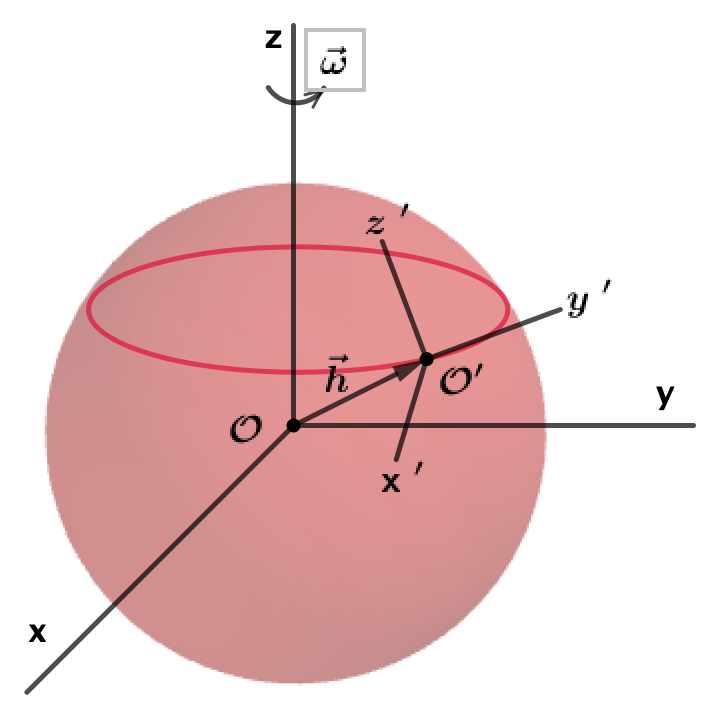
\includegraphics[width=.5\textwidth]{imagenes/imagenes10/T10IM05.png}
\end{figure}
\end{multicols}

Para el caso de que $\mathcal O'$ sea un laboratorio sobre la Tierra, $\omega$ es prácticamente constante por lo que $\dot{\vec \omega} \times \vec r\ '=0$


$\vec a = \vec a\ ' + 2 \vec \omega \times \vec v\ '+ \cancelto{0}{\dot{\vec \omega}\times \vec r \ ' }+ \vec \omega \times (\vec \omega \times \vec r \ ')+ \left( \displaystyle \dv[2]{\vec h}{t} \right)_{\mathcal O}$


$\vec a = \vec a\ ' + 2 \vec \omega \times \vec v\ '+ \vec \omega \times (\vec \omega \times \vec r \ ')+ \vec \omega \times (\vec \omega \times \vec h)$


$\vec a = \vec a\ ' + 2 \vec \omega \times \vec v\ '+ \vec \omega \times [\vec \omega \times (\vec r \ ' + \vec h)]$

$$\boldsymbol{
\vec a = \vec a\ ' + 2 \vec \omega \times \vec v\ '+ \vec \omega \times (\vec \omega \times \vec r)
}$$



Si comparamos este resultado con el del caso de rotación sin traslación en que $\mathcal O$ y $\mathcal O'$ coinciden, el resultado es el mismo. Esto significa que da lo mismo colocar al observador $\mathcal O'$ en la superficie de la tierra que en su centro, con tal de que $\mathcal O'$ gire respecto a $\mathcal O$.

\section{Problemas}
\begin{prob}
Dos trenes A y B se desplazan en rieles paralelos a $70\ \mathrm{km/h}$ y $90\ \mathrm{km/h}$, respectivamente. Calcular la velocidad relativa de B respecto de A cuando el movimiento es en a) el mismo sentido; b) sentido contrario y c) las velocidades forman un ángulo de $60^o$. 	
\end{prob}

\begin{multicols}{2}
	
	$\vec v_A+\vec v_{BA}=\vec v_B; \qquad \vec v_{BA}=\vec v_B-\vec v_A$
	
	a) $ v_{BA}=90-70=20\ \text{km/h}$
	
	b)  $ v_{BA}=90-(-70)=160\ \text{km/h}$
	\begin{figure}[H]
	\centering
	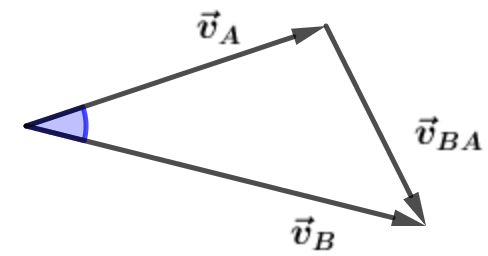
\includegraphics[width=.3\textwidth]{imagenes/imagenes10/T10IM06.png}
\end{figure}
\end{multicols}
c) Teorema del coseno: $\ v_{BA}\sqrt{v_A^2+v_B^2-2v_Av_B\cos 60^o}=170.88\ \text{km/h}$

\begin{prob}
Una persona conduce	un automóvil a través de la tormenta a $80\ \mathrm{km/h}$ y observa que las gotas de lluvia dejan trazos en las ventanas laterales que forman un ángulo de $80^o$ con la vertical. Cuando se detiene, observa que la lluvia cae verticalmente. Calcular la velocidad relativa de la lluvia respecto del coche: a) cuando está detenido y b) cuando circula a $80\ \mathrm{km/h}$.
\end{prob}

\begin{multicols}{2}
	$v_r=v_G-v_c$
	
	$\tan \theta=\dfrac {v_c}{v_G} \to v_G= \dfrac{v_c}{\tan \theta}$
	
	a) $v_G=\dfrac {80}{tan 80^o}=14.107\  \mathrm{km/h}$
	
	b) $v_r=\sqrt{v_c^2+v_G^2}=81.234\  \mathrm{km/h}$
	\begin{figure}[H]
	\centering
	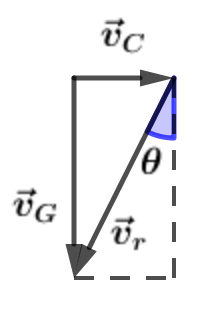
\includegraphics[width=.2\textwidth]{imagenes/imagenes10/T10IM07.png}
\end{figure}
\end{multicols}

\begin{prob}
La brújula de un avión indica que va al Norte y su velocímetro indica que lo hace a $240\ \mathrm{km/h}$. 

a) Si hay un viento de $100\ \mathrm{km/h}$, ?`Cuál es la velocidad del avión relativa a la tierra?

b) ?`Qué rumbo debería tomar el piloto para volar hacia el Norte? ?`Cuál sería su velocidad relativa respecto a la Tierra?
\end{prob}
\begin{figure}[H]
	\centering
	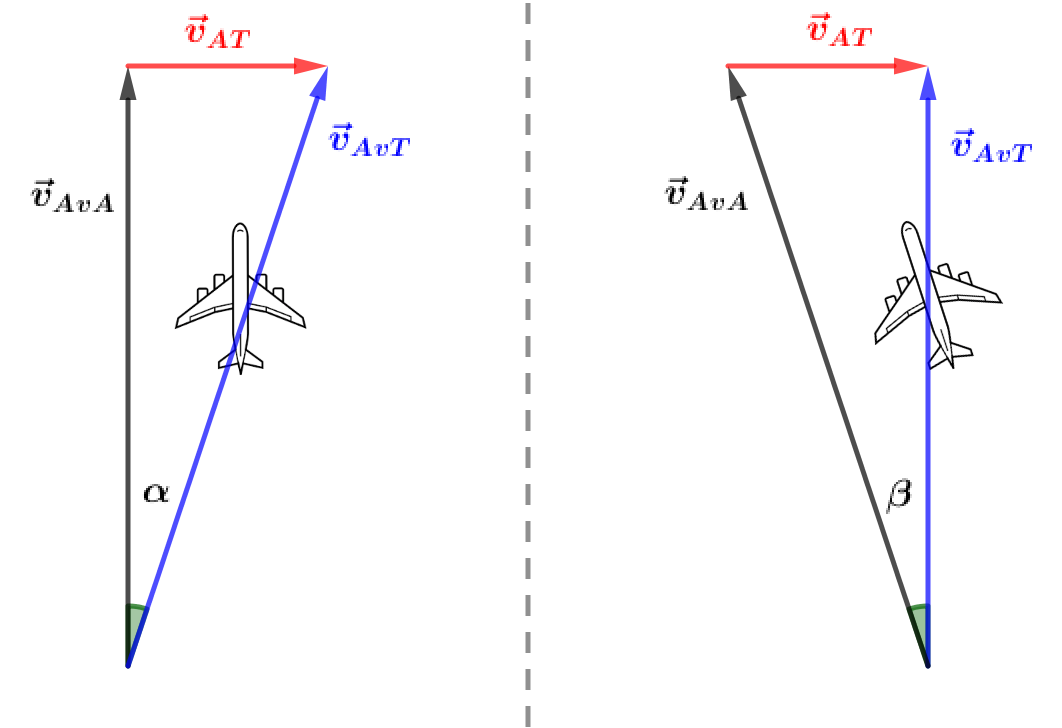
\includegraphics[width=.8\textwidth]{imagenes/imagenes10/T10IM09.png}
\end{figure}

Llamamos $\vec v_{AvT}$ a la velocidad del avión respecto de la Tierra; $\vec v_{AvA}$; la del avión respecto del aire y $\vec v_{AT}$ a la velocidad del aire respecto a la tierra.

--- a) $\vec v_{AvA}=240 \text{km/h};\quad \vec v_{AT}=100\ \text{km/h}$

$\vec v_{AvT}=\vec v_{AvA}+\vec v_{AT}$

$v_{AvT}=\sqrt{240^2+100^2}=260\ \text{km/h}$

$\tan \alpha=\dfrac {v_{AT}}{v_{AvA}}\ \to \ \  \alpha = 23^o $ al Este desde el Norte.

--- b) $\vec v_{AvT}=\vec v_{AvA}+\vec v_{AT}$

Ahora, $\vec v_{AvT}$ es desconocida, pero se dirige al Norte; $\vec v_{AvA}=240$ km/h, pero con dirección $\beta$ desconocida  y $\vec v_{AT}=100$ km/h, en dirección W a E.

$v_{AvT}= \sqrt{240^2-100^2}=218\ $ km/h.

$\sin \beta=\dfrac{v_{AT}}{v_{AvA}}\ to \ \ \beta=25^o$ al Oeste desde el Norte.



\begin{prob}
La posición de una partícula Q en un sistema de coordenadas $\mathcal O$	viene dada por $\vec r=\{ \vec i\ (6t^2-4t)+\vec j\ (-3t^2)+\vec k\ 3\}\ \mathrm{m}$

a) Determinar del sistema $\mathcal O'$ respecto de $\mathcal O$ si la posición de Q medida desde $\mathcal O'$ es $\vec r\ '=\{ \vec i\ (6t^2+3t)+\vec j\ (-3t^2)+\vec k\ 3\}\ \mathrm{m}$.

b) Demostrar que la aceleración de la partícula es la misma en ambos sistemas de referencia.
\end{prob}

\begin{multicols}{2}
	$\vec h=\vec r-\vec r\ '$
	
	$\quad$
	
	$\displaystyle \dv{\vec h}{t} = \vec v_{\mathcal O' \mathcal O}=\dv{\vec r}{t}-\dv{\vec r\ '}{t}$
	\begin{figure}[H]
	\centering
	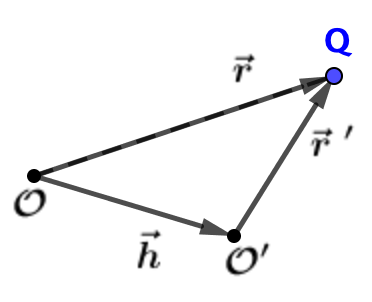
\includegraphics[width=.3\textwidth]{imagenes/imagenes10/T10IM08.png}
\end{figure}
\end{multicols}
a) $\vec v_{\mathcal O' \mathcal O}=[\ \vec i (12t-4)+\vec j (-6t)+\vec k 0 \ ]-[\ \vec i(12t+3)+\vec j(-6t)+\vec k 0  \ ]=-7\vec i\ \text{m}$

b) $\displaystyle \dv{\vec v_{\mathcal O' \mathcal O}}{t}=\vec a -\vec a \ '=0 \to \vec a=\vec a \ '$

%********************************************************
\newpage %***********************************************
\begin{myblock}{Relatividad de Galileo.}
\begin{small}
\vspace{2mm} Se entiende por la teoría de la relatividad clásica o relatividad de Galileo al estudio del movimiento de una partícula condicionado a un sistema de referencia arbitrariamente escogido. De este modo se establece que la percepción y la medida de las magnitudes físicas varían en función al sistema de referencia escogido. Para poner un ejemplo: no es lo mismo observar la caída de una manzana que está moviéndose en un tren si lo vemos desde fuera del tren (la manzana hace una parábola) o desde dentro (la manzana cae en vertical).

\vspace{2mm} Esta dependencia de la percepción del movimiento según el sistema de referencia escogido es lo que se conoce como relatividad clásica. Fue descrita por Galileo Galilei en el ejemplo del barco que aparece en sus Diálogos sobre los dos máximos sistemas del mundo en el siglo XVII.

\vspace{2mm} Su famosa frase: Eppur si muove (``Y sin embargo se mueve’’) es el resumen de la mentalidad de la época ante un hecho actualmente reconocido. La Tierra se mueve alrededor del Sol, si bien sus habitantes no percibimos que esta alcanza velocidades de hasta 106.000 km/h pues nosotros mismos nos movemos a esa velocidad. 

\vspace{2mm} Esta teoría de la relatividad clásica se conoce también como invariancia galileana y es el primer paso hacia la realidad física más general que se conoce como teoría de la relatividad especial desarrollado por Albert Einstein en 1905.

\vspace{2mm} La teoría clásica de la relatividad establecía que las magnitudes físicas eran dependientes del sistema de referencia escogido pero presuponía que el tiempo era un ente absoluto e independiente del sistema de referencia escogido. Sin embargo en el siglo XX, tras el experimento de Michelson y Morley quedó demostrada la invariabilidad de la velocidad de la luz lo cual condujo al descubrimiento de la relatividad de ambos espacio y tiempo.

\vspace{2mm} Los descubrimientos de Galileo sobre la relatividad de las percepciones de la realidades físicas espaciales ante distintos sistemas de referencia supusieron una auténtica revolución en su época.	
\end{small}
\end{myblock}
